\chapter{Forth Kommunikation}
\label{chap:forthcommunication}

In diesem Kapitel wird beschrieben, wie die Entwicklungsumgebung mit dem Forth-Prozess kommuniziert. Die Kommunikation mit dem Forth-Prozess ist von zentraler Bedeutung, da die Funktionalität der Entwicklungsumgebung davon abhängt, ob die Kommunikation stabil läuft. Es wird gezeigt, wie die Kommunikation entworfen, implementiert und getestet wurde.

\section{Prozess Kommunikation}
Um mit dem Prozess zu kommunizieren, gibt es die Möglichkeiten: ein Machine Interface zu implementieren, oder direkt mit dem Prozess zu kommunizieren. In den folgenden Kapiteln werden die beiden Möglichkeiten kurz beschrieben.

\subsection{GDB/MI-Commands}

Eine Möglichkeit, mit dem Prozess zu kommunizieren, ist der Gebrauch, eines Machine Interfaces (MI), wie es für den GDB implementiert wurde. GDB/MI ist ein linienbasiertes, maschinenorientiertes Text-Interface zum GDB. Es wurde entwickelt, um den GDB, als Debugger, in ein grössers System einfacher einzubinden.\cite{gdb} Ein MI ähnliches Interface wäre mit grossem Aufwand verbunden, da das Interface zuerst definiert werden müsste. Dafür könnte aber der CDT-Debugging-Mechanismus verwendet werden, da der CDT-Debugger auf dem GDB/MI basiert. Auch ist der CDT-Debugger sehr kompliziert\cite{mieclipse} und es wäre ein grosser Einarbeitungsaufwand notwendig, den Forth Debugger darauf aufzubauen.\cite{mieclipse}

\subsection{Direkte Kommunikation mit dem Prozess}

Eine weitere Möglichkeit besteht darin, die Befehle direkt an den Prozess zu senden und auf Antworten zu warten. Dafür müssen einige Klassen implementiert werden, um die Kommunikation zu vereinheitlichen und zu vereinfachen.

\subsubsection{Probleme bei der Kommunikation}

Bei der Kommunikation mit dem Prozess können einige Probleme auftreten: Es kann sein, dass der Prozess plötzlich keine Antworten mehr gibt. Auch weiss man nicht, wie lange es dauern wird, bis der Prozess Antwort gibt. Diese Probleme müssen mit den oben genannten Klassen gelöst werden.

\section{Kommunikation}

Ich habe mich dafür entschieden, die Kommunikation nicht über ein MI-Interface zu implementieren. Der Aufwand, ein solches Interface zu entwerfen und zu implementieren, sowie die Einarbeitungszeit für den CDT-Debugger, wären zu gross. Die Kommunikation wird also direkt mit dem Prozess erfolgen. Das Design und die Implementation wird in den folgenden Kapiteln besprochen.

\section{API-Design}

In einem ersten Schritt wurde ein API entworfen, das die Kommunikation mit dem Prozess möglichst einfach halten soll.

\begin{figure}[H]
	\centering
		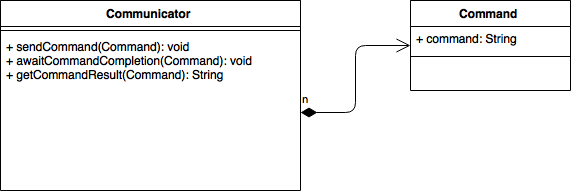
\includegraphics[scale=0.6]{forthcommunication/api.png}
		\caption{Ein erstes Design des Prozess-API. Die zentrale Kommunikation geschieht über die Communicator-Klasse. Es können Befehle gesendet und Resultate abgewartet werden.}
		\captionsetup{margin=0cm,font={footnotesize}}
		\label{fig:api}
\end{figure}

\section{Implementierung}

Bei der Implementierung kamen Änderungen hinzu. Im folgenden Klassendiagramm sind die Änderungen ersichtlich. Danach wird die Klassenstruktur genauer erläutert.

\begin{sidewaysfigure}[p]

	\centering
		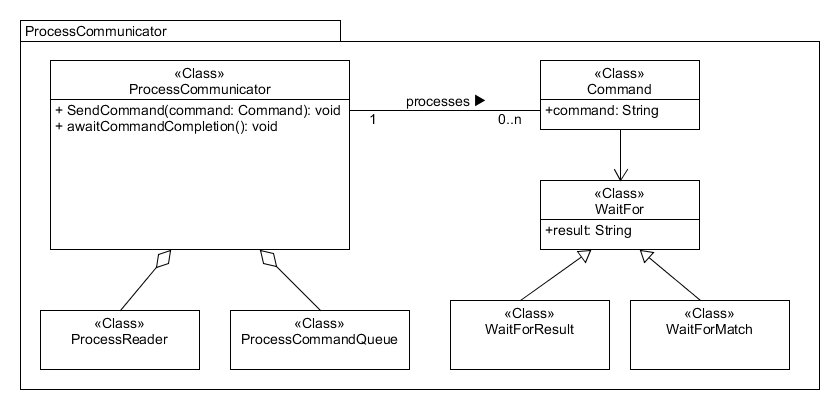
\includegraphics[scale=0.75]{forthcommunication/communicator.png}
		\caption{Klassendiagramm des ProcessCommunicators.}
		\captionsetup{margin=0cm,font={footnotesize}}
		\label{fig:communicator}

\end{sidewaysfigure}

\newpage

\subsection{Klassenbeschreibung}

Über das \verb!ProcessCommunicator!-API können Befehle an den Prozess gesendet werden. Das API stellt blockierende und nicht blockierende Methoden für das Senden von Befehlen zur Verfügung. So können Befehle über die \verb!sendCommand! Funktion einen \verb!Command! senden, ohne zu blockieren. Falls auf ein bestimmtes Resultat gewartet werden muss, kann die Funktion \verb!sendCommandAwaitResult! verwendet werden, die den aufrufenden Thread blockiert, bis das Resultat eingetroffen ist. 

\subsubsection{ProcessCommunicator}

Der \verb!ProcessCommunicator! ist die zentrale Kommunikationsstelle. Über den \\ \verb!ProcessCommunicator! können die \verb!Commands! gesendet und gleichzeitig die angeforderten Resultate warten abgewartet werden.

\subsubsection{ProcessReader}

Der \verb!ProcessReader! ist eine verschachtelte Klasse des \verb!ProcessCommunicator!, der als Thread im Hintergrund den Stream des Prozesses liest und verarbeitet. Der \verb!ProcessReader! notifiziert alle Threads, die auf ein Resultat warten, sobald dieses eingetroffen ist.

\subsubsection{ProcessCommandQueue}

Die \verb!ProcessCommandQueue! ist eine verschachtelte Klasse des \verb!ProcessCommunicator!, die als Thread im Hintergrund Befehle verarbeitet und an den Prozess sendet. Die \verb!ProcessCommandQueue! blockiert, falls dies von einem \verb!Command! spezifiert wurde. Wenn die \verb!ProcessCommandQueue! blockiert, werden keine weiteren Befehle mehr verarbeitet, bis das von der \verb!WaitFor!-Klasse spezifizierte Resultat vom Prozess geschrieben wurde.

\subsubsection{Command}

Die \verb!Command!-Klasse repräsentiert einen Befehl, der über den \verb!ProcessCommunicator! an den Prozess gesendet werden kann. In einem Command kann ein \verb!WaitFor! spezifiziert werden, falls der \verb!Command! blockieren soll, bis ein Resultat vom Prozess geliefert wird.

\newpage
\subsubsection{WaitFor}

Mit der abstrakten \verb!WaitFor!-Klasse können Resultate des Prozesses abgewartet werden. Dafür wurden verschiedene Implementationen bereitgestellt. Mit der \verb!WaitForResult! kann String-Resultate abgewartet werden. Mit der \verb!WaitForMatch!-Klasse kann per Regex ein Resultat abgewartet werden. Im folgenden Pseudocode wird die Funktionalität der \verb!WaitForMatch!-Klasse im Zusammenhang mit dem senden eines \verb!Commands! gezeigt.
%
\begin{verbatim}
sendCommandAwaitMatch("foo", "[1-9]")
\end{verbatim}
%
Der aktuelle Thread wird blockiert, bis der Prozess eine Ziffer zwischen 1 und 9 schreibt. Für das Warten auf ein Resultat wurde ein Timeout implementiert. Falls der Prozess in der vorgegebenen Zeit keine Antwort gibt, wird eine \\ \verb!CommandTimeOutException! geworfen und der \verb!ProcessCommunicator! wird heruntergefahren, um das Senden weiterer Befehle zu verhindern.

\section{Testing}
Der \verb!ProcessCommunicator! wurde vor allem mit Unit-Tests getestet. Unter diesen Tests befindet sich ein Stresstest, welcher möglichst viele Befehle an den Prozess sendet.

